\subsection{Community Support}

{
\setbeamertemplate{background canvas}{\tikz[remember picture]\node[opacity=0.7] at (current page.center) {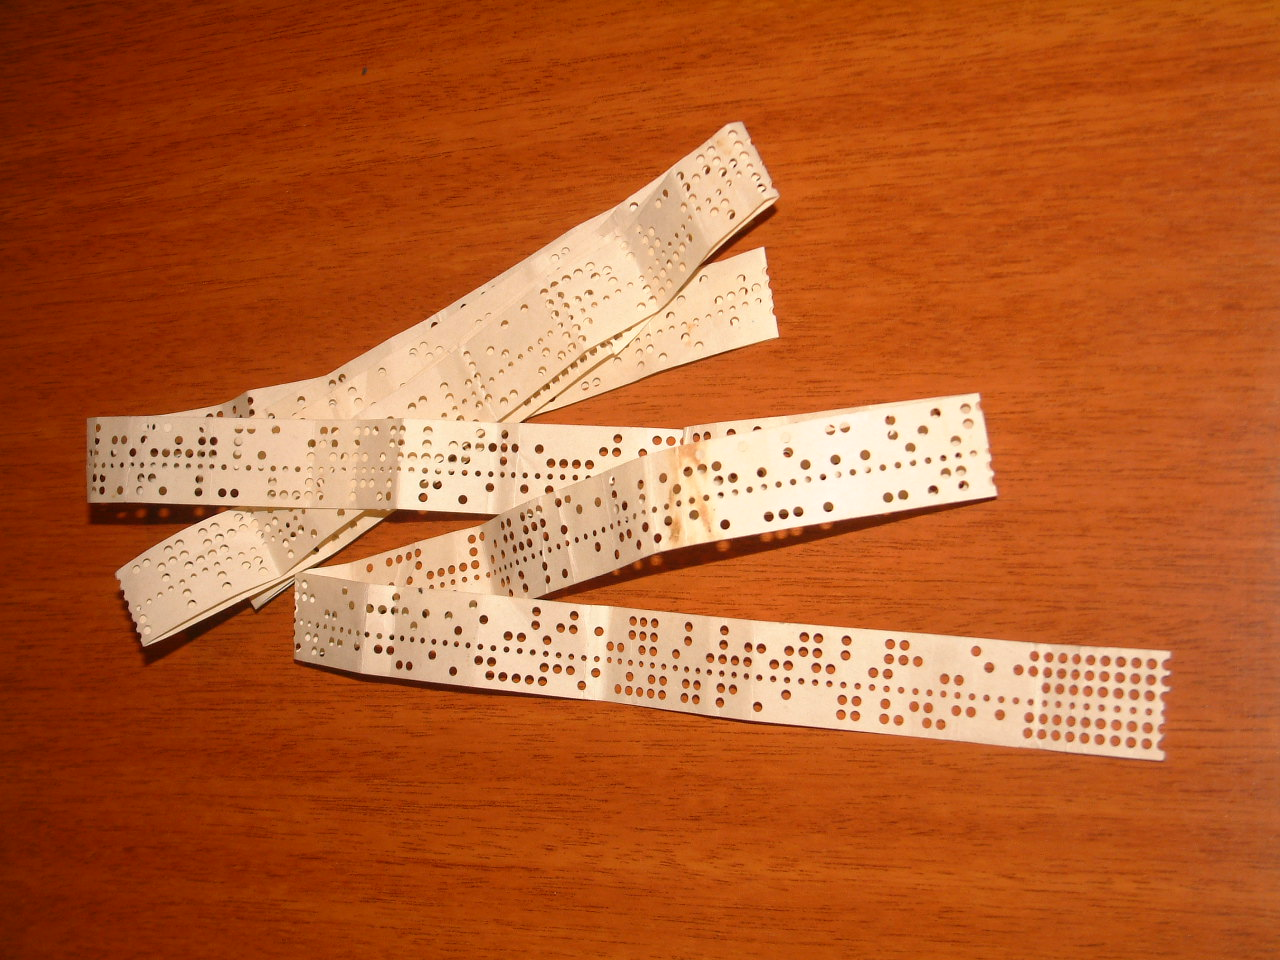
\includegraphics[height=1.05\textheight,keepaspectratio]{nontex/illustrations/baudotTape.jpg}};}
\begin{frame}
\frametitle{How Does The Community Prefer To Represent Regexes?}
\begin{block}{\begin{Large}Knowledge Of Community Standards Is Missing\end{Large}}
\begin{itemize}
\item \begin{large}programmers probably choose the best representation\end{large}
\item \begin{large}conformance to community standards eases comprehension\end{large}
\end{itemize}
\end{block}
\end{frame}
}
\note[itemize]{
    \item https://i.ytimg.com/vi/Gt-5lS9hJFA/hqdefault.jpg
        \item cite that fact!
}

%------------------------------------------------


\begin{frame}
\frametitle{Another Point}
\end{frame}
\note[itemize]{
    \item pt 1
    \item pt 2
}

%------------------------------------------------
